\chapter{Indústria 4.0 e Internet das Coisas}
\label{chapter:industria_4_0_iot}

A revolução dos dados atingiu praticamente todas as áreas de engenharia elétrica, desde a eletrônica, desenvolvendo dispositivos capazes de receber dados telemétricos, processa-los e envia-los para demais hubs, a servidores de armazenamento de dados, recorrentemente chamados de Data Warehouses. Esse conjunto de mudanças engloba a Indústria 4.0, uma indústria que capta dados de suas máquinas em tempo real em larga escala, analisa, armazena, e utiliza inteligência artificial e estatística, para tomada de decisões estratégicas, contando sempre , é claro, com ajustes humanos.

\section{Internet das Coisas}
\label{section:iot}

"A Internet das Coisas tem o potencial de mudar o mundo. Assim como a Internet fez. Talvez até mais"\cite{ashton:iot}. Uma tradução livre de Rampim \cite{Rampim:iot} da frase de Kevin Ashton, cofundandor do Auto-ID Center, em 1999. Apesar de ser um nome feito somente para chamar atenção, foi a primeira citação da expressão Internet das Coisas, e de lá vingou.

Dentre o meio da Indústria 4.0, encontra-se a internet das coisas ou IoT, responsável por estruturar as aplicações de aquisição, transmissão e armazenamento de dados a serem analisados. Não é uma surpresa que este setor envolva áreas como eletrônica, computação e telecomunicações em um pacote só. De fato suas camadas são mundos diferentes interligados a um propósito : transmitir dados sobre um dispositivo e/ou para um dispositivo em tempo real. Segundo a Cisco IBSG \cite{cisco:ibsg}, há mais objetos conectados que a própria população mundial, fazendo com que o ano de 2009 ser considerado o ano de nascimento do IoT.

Pode-se definir IoT como a estrutura que comunica dispositivos em rede, permitindo a transmissão de dados sobre estes em tempo real. É a ponte que permite a troca de informações sobre um dispositivo, qual seu status, seu desempenho, suas condições físicas e do ambiente ao seu redor. Mas, para que este ciclo esteja completo é necessário camadas que desempenham tarefas específicas, para que o dado chegue a quem ou a o que está esperando.

\section{Visão geral de uma aplicação IoT}
\label{section:overview}

Observe  a \ref{fig:1.1.0/iot_app}, temos uma rede de N sensores que enviam dados telemétricos e N atuadores que recebem ordens para executar uma função, ambos estão em rede e podem receber e enviar informação em tempo real. O servidor, que pode ser um Broker como será descrito mais tarde neste trabalho, encaminha os dados (ou mensagens) para as aplicações do banco de dados, que é utilizado para Análise destes e recebe informações do controlador, que por sua vez envia mensagens de decisões baseada na análise de dados de alguma forma estas são transmitidas para os atuadores.

\begin{figure}[h!]
\centering
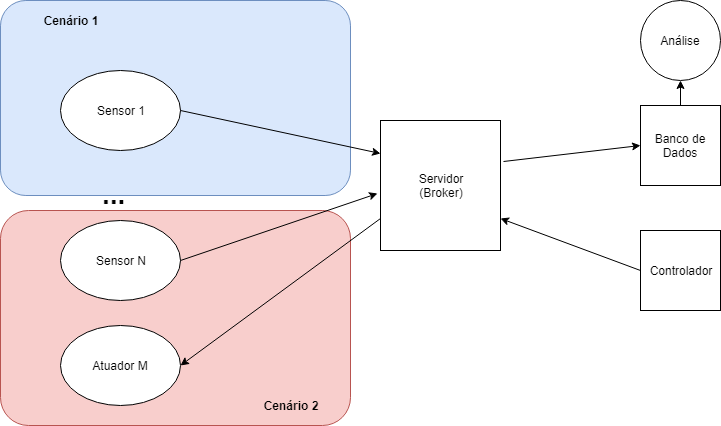
\includegraphics[width=10cm]{./02_Capitulos/02_Cap1/figures/iot_app}
\caption{Um exemplo de aplicação IoT que percorre os problemas a solucionar}
\label{fig:1.1.0/iot_app}
\end{figure}

Porém o sensor 1 está localizado em um determinado cenário com usas próprias características físicas e de rede, assim como outros estão em outro cenário. Supondo que o primeiro seja uma rede com poucos sensores e o segundo cenário seja uma rede com um grande fluxo de dados, sujeito a congestionamento. Seria uma grande ajuda que o  sistema se ajustasse a estas mudanças de cenário.

Este trabalho visa implementar um sistema que utiliza o protocolo de aplicação MQTT\ref{subsection:mqtt}, para transmissão de dados em tempo real entre dispositivos, oferecendo suporte a plataformas embarcadas e para consoles com sistemas operacionais (Linux, Windows). O sistema contempla também persistência de dados utilizando banco de dados MongoDB \ref{subsection:bancos_IoT}, com o diferencial de se adaptar a cenários através de canais de dados chamados Data Streams, oferecendo diferentes configurações que podem otimizar o envio de dados em cada cenário.

\begin{figure}[h!]
\centering
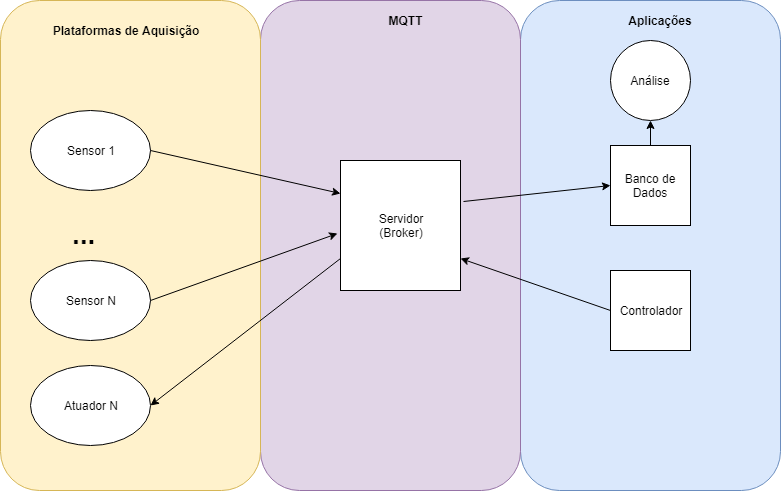
\includegraphics[width=10cm]{./02_Capitulos/02_Cap1/figures/iot_app-layers}
\caption{Como a camada IoT se encaixa na aplicação}
\label{fig:1.1.0/iot_app-layers}
\end{figure}


O sistema percorre toda a camada de IoT como na \ref{fig:1.1.0/iot_app-layers}, da aquisição de dados a persistência destes, para entender melhor esta camada, iremos descrever o projeto e implementação em cada passo do sistema.

\section{As Camadas do IoT}
\label{section:camadas_iot}

Semelhante a camada de rede, a camada de IoT também exerce funções específicas no transporte de dados, e a camada acima não necessariamente precisa saber como a inferior funciona, somente precisa dos dados que esta camada entrega e executar suas tarefas sobre estes até chegar ao destino especificado, formando uma estrutura de pilha como na figura \ref{fig:1.2.0/camadas_iot};

\begin{figure}[h!]
\centering
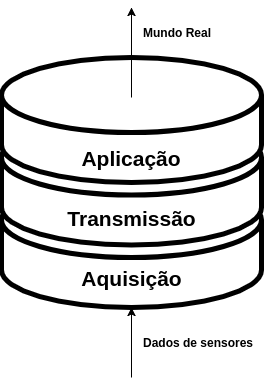
\includegraphics[width=5cm]{./02_Capitulos/02_Cap1/figures/iot_stack}
\caption{As três camadas do IoT, dos sensores ao mundo real}
\label{fig:1.2.0/camadas_iot}
\end{figure}

A primeira camada é a de aquisição de dados, que lida com o mundo físico e amostra estes dados através de sensores e conversores A/D, também realiza o processamento para entregar em um formato adequado para transmissão e entendível do outro lado, dependo da aplicação. A segunda camada é a camada de transmissão, onde estão, efetivamente, as camadas de rede embutidas. Como o nome já denuncia, ela lida com os aspectos de rede e comunicação para que o dados cheguem as seus destinos. E por último temos a camada de aplicação, a mais abrangente e que envolve maior poder computacional. Ela recebe os dados e lida com os processos de aplicação destes dados, seja análise, visualização, armazenamento ou a estruturação destes.

\subsection{Aquisição}
\label{subsection:aquisicao}

A etapa de aquisição está inserida diretamente no contexto de dados físicos, geralmente são hardwares menos complexos, focados em processamento de dados e entrada e saída com conversão analógico-digital. Se comunicam com sensores ou centrais de controle lógico. São responsáveis por:

\begin{itemize}
	\item Receber dados de sensores;
	\item conversão A/D;
	\item Processamento e calibragem de valores;
	\item Envio de dados em tempo real;
\end{itemize} 

Para atender essas tarefas, não é necessário grande poder de processamento, microcontroladores ou microprocessadores são capazes de atender tais necessidades se acompanhados de módulos de rede e portas I/O, assim como a implementação do software. Veremos dois exemplos no capítulo de implementação do projeto, que utilizam tanto MCU (Micro-Controller Units) ou Consoles com Sistemas Operacionais leves.
 

\subsection{Transmissão}
\label{subsection:transmicao}

Esta camada é o coração do IoT. A forma de transmissão define quais dispositivos eletrônicos e qual sua especificação técnica necessária para os quesitos de transmissão. Também define como os softwares da camada de aplicação e aquisição devem ser implementados baseado na estrutura da pilha de rede que será usada para transmitir.

Na próxima seção, veremos sobre a camada de rede e suas diversas formas de implementação. É importante que esta camada seja definida da melhor forma a atender sua aplicação, atendendo aspectos: 
\begin{itemize}
\item quantidade de dados transmitido;
\item número de acessos; 
\item distância entre dispositivos;
\item segurança;
\end{itemize}

\subsection{Aplicação}
\label{subsection:aplicacao}

A camada de aplicação encabeça a pilha do IoT. É ela que de fato trata os dados e realiza as aplicações deste. Ela disponibiliza os dados para o mundo real, podendo exercer múltiplas funções simultâneas incluindo:

\begin{itemize}
\item Armazenamento e Análise;
\item Visualização; 
\item Inteligência e aprendizado;
\item Serviços e servidores;
\item Gerenciamento e configuração;
\end{itemize}

Nesta camada estão presentes os endpoints apontados pela camada de aquisiçao, o destino dos dados. Bem assim como os servidores que gerenciam os clientes (geralmente implementados na camada de aquisição) e serviços e configurações oferecidos pelo sistema em si.

\section{Camadas de Rede}
\label{section:camadas_de_rede}

Como visto anteriormente, a camada de transmissão basicamente define a infraestrutura do sistema. Ela é construído com as camadas de rede como base. Portanto definir as camadas de rede e seus protocolos é definir a camada de transmissão em si.

Redes de computadores são complexas com diferentes aspectos a se preocupar. Dividir em camadas permite modularizar a implementação da rede, de modo que cada camada tenha uma tarefa na estrutura de comunicação dos aspectos físicos ao software. Como a camada de cima não precisa saber sobre os detalhes e especificações da camada de baixo, as mudanças de uma parte do sistema é transparente para o resto do sistema. Existem diversas formas de implementação de camadas, mas todas se baseiam em um modelo de referência, o modelo OSI \cite{Zimmermann:1988:ORM:59309.59310}.


\begin{figure}[h!]
\centering
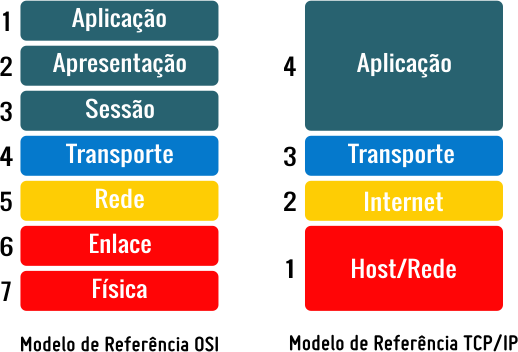
\includegraphics[width=8cm]{./02_Capitulos/02_Cap1/figures/modelo_osi_tcpip}
\caption{Diferenças entre OSI e TCP/IP em suas camadas}
\label{fig:1.2.0/modelo_osi_tcpip}
\end{figure}

Baseado no modelo OSI. Temos o modelo TCP/IP \cite{TCPIP}, visualizado em \ref{fig:1.2.0/modelo_osi_tcpip} e utilizado na internet e base para protocolos de aplicação muito utilizados como HTTP, WebSocket e MQTT. Em ambos cada camada exerce uma tarefa com seu respectivo protocolo, como resumido na tabela \ref{table:1.2.0}.

\begin{table}[h]
\centering
\caption{As camadas e e suas funções}
\begin{tabular}{|l|l|}
\hline
\multicolumn{1}{|c|}{CAMADA} & \multicolumn{1}{c|}{DETALHES}                                                  \\ \hline
7 - Aplicação                & Define instruções específicas da aplicação          						    \\ \hline
6 - Apresentação             & Formatação dos dados, conversão dos dados                     					\\ \hline
5 - Sessão                   & Negociação e conexão com outros nós, analogia                                \\ \hline
4 - Transporte               & Oferece métodos para a entrega de end-to-end                        			\\ \hline
3 - Rede                     & Roteamento de pacotes em uma ou várias redes                                 \\ \hline
2 - Enlace                   & Detecção de erros;                                                            \\ \hline
1 - Física                   & Aspectos físicos da transmissão \\ \hline
\end{tabular}
\label{table:1.2.0}
\end{table}


O foco desta literatura está na camada de aplicação e suas funcionalidades. Apesar de diferentes tecnologias utilizarem diferentes camadas abaixo, serão especificas características de protocolos construídos em cima do TCP/IP, por seu uso na Internet e redes industriais, e que sejam eficientes em trocas de mensagens em tempo real.

